% mn2esample.tex
%
% v2.1 released 22nd May 2002 (G. Hutton)
%

%
%  Notes on 20 Apr 2012
%  Having trouble with bibliography; mn2e style file will not recognize abbreviations for strings. Importing as mn-jour.bib file does not work. 
%  Fixed by using macro definition with new commands, but these need to be uncommented in blazarenv_macros.tex 
%  
%  mn2e file also overwrites long author lists; stated that this is a known bug, but not fixed (grr). 
%  
%  Manually modifying long entries:
%   
% \bibitem[\protect\citeauthoryear{{Blanton}, {Hogg}, {Bahcall}, {Brinkmann},
%   {Britton}, {Connolly}, {Csabai}, {Fukugita}, {Loveday}, {Meiksin}, {Munn},
%   {Nichol}, {Okamura}, {Quinn}, {Schneider}, {Shimasaku}, {Strauss}, {Tegmark},
%   {Vogeley} \& {Weinberg}}{{Blan]{bla03a}
% {Blanton} M.~R.,  {Hogg} D.~W.,  {Bahcall} N.~A.,  {Brinkmann} J.,  {Britton}
%   M.,  {Connolly} A.~J.,  {Csabai} I.,  {Fukugita} M.,  {Loveday} J.,
%   {Meiksin} A.,  {Munn} J.~A.,  {Nichol} R.~C.,  {Okamura} S.,  {Quinn} T.,
%   {Schneider} D.~P.,  {Shimasaku} K.,  {Strauss} M.~A.,  {Tegmark} M.,
%   {Vogeley} M.~S.,    {Weinberg} D.~H.,  2003, \apj, 592, 819
% 
% to
% 
% \bibitem[\protect\citeauthoryear{{Blanton}, {Hogg}, {Bahcall}, {Brinkmann},
%   {Britton}, {Connolly}, {Csabai}, {Fukugita}, {Loveday}, {Meiksin}, {Munn},
%   {Nichol}, {Okamura}, {Quinn}, {Schneider}, {Shimasaku}, {Strauss}, {Tegmark},
%   {Vogeley} \& {Weinberg}}{{Blanton} et~al.}{2003}]{bla03a}
% {Blanton} M.~R.,  et~al.  2003, \apj, 592, 819
% 
% and
% 
% \bibitem[\protect\citeauthoryear{{Plotkin}, {Anderson}, {Brandt},
%   {Diamond-Stanic}, {Fan}, {Hall}, {Kimball}, {Richmond}, {Schneider},
%   {Shemmer}, {Voges}, {York}, {Bahcall}, {Snedden}, {Bizyaev}, {Brewington},
%   {Malanushenko}, {Malanushenko}, {Oravetz}, {Pan} ]{plo10}
% {Plotkin} R.~M.,  {Anderson} S.~F.,  {Brandt} W.~N.,  {Diamond-Stanic} A.~M.,
%   {Fan} X.,  {Hall} P.~B.,  {Kimball} A.~E.,  {Richmond} M.~W.,  {Schneider}
%   D.~P.,  {Shemmer} O.,  {Voges} W.,  {York} D.~G.,  {Bahcall} N.~A.,
%   {Snedden} S.,  {Bizyaev} D.,  {Brewington} H.,  {Malanushenko} V.,
%   {Malanushenko} E.,  {Oravetz} D.,  {Pan} K.,    {Simmons} A.,  2010, \aj,
%   139, 390
% 
% to
% 
% \bibitem[\protect\citeauthoryear{{Plotkin}, {Anderson}, {Brandt},
%   {Diamond-Stanic}, {Fan}, {Hall}, {Kimball}, {Richmond}, {Schneider},
%   {Shemmer}, {Voges}, {York}, {Bahcall}, {Snedden}, {Bizyaev}, {Brewington},
%   {Malanushenko}, {Malanushenko}, {Oravetz}, {Pan}, {Simmons}}{{Plotkin} et~al.}{2010}]{plo10}
% {Plotkin} R.~M.,  et~al.  2010, \aj,
%   139, 390
% 
%  
%  
%  

\documentclass[useAMS,usenatbib]{mn2e}

\usepackage{graphicx}
\usepackage{verbatim}
\usepackage{natbib}
\usepackage{amsmath}
\bibliographystyle{mn2e}

%%%%% AUTHORS - PLACE YOUR OWN MACROS HERE %%%%%

\input blazarenv_macros.tex	

%%%%%%%%%%%%%%%%%%%%%%%%%%%%%%%%%%%%%%%%%%%%%%%%

\title[Clustering properties of blazars]{Environmental And Clustering Properties Of Blazars From The Sloan Digital Sky Survey}
\author[K.W. Willett, T.J. Nelson, \& L.F. Fortson]{K.W. Willett$^{1}$\thanks{E-mail: willett@physics.umn.edu}, T. J. Nelson$^{1}$, L. F. Fortson$^{1}$\\
$^{1}$School of Physics and Astronomy, University of Minnesota, Minneapolis, MN 55455, USA}
\begin{document}

\date{Accepted 1988 December 15. Received 1988 December 14; in original form 1988 October 11}

\pagerange{\pageref{firstpage}--\pageref{lastpage}} \pubyear{2012}

\maketitle

\label{firstpage}

\begin{abstract}
We present results from a large-scale study of the megaparsec-scale environments of blazars, including BL Lac objects and flat-spectrum radio quasars. Using the catalog of galaxies from the Sloan Digital Sky Survey DR8 catalog, we compute spatial covariance amplitudes for a sample of more than 2900 blazars, the largest ever assembled. The covariance amplitudes are analyzed to compute the relative levels of clustering for various blazar types. We also compare the clustering of blazars to FR~I and FR~II radio galaxies to explore possibility of a parent population in the context of a blazar sequence. Finally, we present preliminary results on the morphologies of galaxies located within 1~Mpc of blazars, with classifications supplied by Galaxy Zoo data.
\end{abstract}

\begin{keywords}
blazars -- active galactic nuclei: environment.
\end{keywords}

\section{Introduction} \label{sec-intro}

%%%%%%%%%%%%
%%% INTRODUCTION
%%%%%%%%%%%%

The standard model of blazars presumes that they are active galaxies with a jet closely aligned to the observer's line of sight. Observationally, blazars can be distinguished from other active galaxies with a variety of diagnostics, including extreme luminosities and non-thermal spectra dominated by relativistic beaming. 

The population of blazars displays significant observational diversity, however. The primary historical method of classification has been through the optical spectrum of the blazar, dividing them into two groups: (1), BL Lacs, characterized by weak or non-existent optical emission lines, and (2) flat-spectrum radio quasars (FSRQs), which have strong, broad emission lines in their optical spectrum. An enduring question for many years has been whether BL Lacs and FSRQs comprise physically distinct populations of galaxies, or whether a sequence exists between the two groups. 

Since highly-beamed emission from the relativistic jet often dominates the light observed from the blazar, studies of the object itself are challenging. As an alternative approach, we study the clustering properties of blazars in an attempt to determine their parent populations. Clustering studies benefit from the fact that they are assumed to be independent of the blazar's orientation to our line-of-sight. Differences in the clustering properties on scales of hundreds of kpc are already known to exist, for example, in the density-morphology relation \citep{dre80} and in the populations of powerful radio galaxies \citep{pre88}. 

Previous clustering studies of blazars have been limited by sample sizes of only a few tens. With the release of the Sloan Digital Sky Survey (SDSS), we have for the first time a large and deep catalog with nearly uniform photometry and coverage out to redshifts greater than 1. We combine the SDSS data with the latest identifications of blazars, for which counts are now in the thousands. The larger sample size allows for the first time robust classification of blazar clustering properties, which we compare to other samples to explore possible parent populations.

\citet{wur97} carried out a deep, largely subarcsec imaging survey of BL Lac objects conducted at the CFHT. \citet{wur93} described the results pertaining to the host galaxies of 50 BL Lac objects at $z<0.65$; \citet{wur97} report on the clustering environment of 45 of these 50 BL Lacs. The remaining five objects either have unknown or very uncertain redshifts or we were unable to obtain deep, photometrically calibrated images of them, which prohibited successful clustering analysis.  

With this substantially larger (45 vs. 5) sample, we have confirmed the early result of \citet{pre88} that BL Lac objects largely avoid rich clusters at low redshift and have distributions in $B$ richness measurements much more consistent with those of FR~II radio galaxies than with FR~I's.  The typical environment of a BL Lac object is a sub-Abell richness class 0 cluster with a CFHT sample mean of $\langle$\bgb$\rangle=209$~Mpc$^{1.77}$. Further, these results apply to all types of BL Lac objects regardless of selection method (e.g., radio or X-ray selection) or detailed property (e.g., high or low optical polarization percentage, presence/absence of emission lines etc.) because no BL Lac subtype has statistically distinct \bgb~values. The only exceptions to this statement are correlations between redshift and \bgb~and between host galaxy luminosity and \bgb, and a possible anticorrelation between \bgb~and radio core dominance. 

\citet{smi95} computed \bgb~for a sample of 16 BL~Lac galaxies and six FR~I galaxies; the correlation amplitudes for the two samples were statistically indistinguishable for the small sample sizes, and were consistent with an Abell richness class of 0. 

\citet{lie11} examined the megaparsec-scale environments of active galaxies at $z<0.4$ by constructing a luminosity-density field based on luminous red galaxies in the SDSS. They showed that radio galaxies tended to exist in overdensities on scales of 3~$h^{-1}$~Mpc. BL~Lacs were primarily found in low-density environments, but were also found in high-density regions. Radio-loud quasars were found in low-density environments as compared to their LRG environment. 

%%%%%%%%%%%%
%%% SAMPLE
%%%%%%%%%%%%

\section{Measuring the clustering properties}\label{sec-data}

Clustering environment can characterized using the spatial covariance amplitude method first developed by \citep{lon79}. For any population of objects as viewed on the sky in the far-field limit, its angular distribution can be approximated by:

\begin{equation}
\label{eqn-angcov}
n[\theta]d\Omega = N_g (1 + w[\theta]) d\Omega,
\end{equation}

\noindent where $n[\theta]d\Omega$ is the number of galaxies in a ring of solid angle $d\Omega$ at angular distance $\theta$ from the center of the ring. $N_g$ is the number of background galaxies in the ring, and the factor of $(1+w[\theta])$ expresses the probability of finding additional galaxies over the background level. $w[\theta]=0$ would correspond to a uniform angular distribution of galaxies in the universe (no clumping). 

The standard assumption, confirmed with deep optical observations of field galaxies, is that the angular distribution of galaxies follows a power law such that:

\begin{equation}
\label{eqn-wtheta}
w[\theta] = A\theta^{1-\gamma},
\end{equation}

\noindent where $A$ is the angular covariance amplitude and $\gamma$ an index describing the slope of the power-law distribution. We assume the canonical value of $\gamma=1.77$. The amplitude of $A$ for a particular system, then, determines the degree of clustering with respect to other similarly-scaled structures in the universe. 

Since this derivation has been completely general so far, we note that subscripts are used with computing the covariance amplitudes to indicate the type of object measured. For instance, $A_{gg}$ represents the galaxy-galaxy correlation amplitude, while $A_{gB}$ is the galaxy-BL~Lac correlation amplitude. 

Without a distance dependence, $A$ can be computed for any point on the sky by simply integrating Equation~\ref{eqn-angcov} from 0 out to $\theta$. This gives:

\begin{equation}
\label{eqn-angint1}
\int^\theta_0 n[\theta^\prime]d\Omega = \int^\theta_0 N_g (1 + w[\theta^\prime]) d\Omega.
\end{equation}

\noindent The solid angle subtended by an angle of $2\theta$ is $\Omega=2\pi(1-cos[\theta])$; for $\theta\ll1$, this translates to a differential:

\begin{equation}
d\Omega \simeq 2\pi \theta d\theta.
\end{equation}

\noindent Integrating Equation~\ref{eqn-angint1} over the angle yields:

\begin{eqnarray}
\int^\theta_0 n[\theta^\prime] 2 \pi \theta d\theta & = & \int^\theta_0 N_g (1 + w[\theta^\prime]) 2 \pi \theta d\theta \\
2\pi \int^\theta_0 \theta^\prime n[\theta^\prime]d\theta & = & 2 \pi N_g \int^\theta_0 \theta^\prime (1 + A {\theta^\prime}^{1-\gamma}) d\theta \\
N_t \left(\frac{\theta^2}{2}\right) & = & N_g \left(\frac{\theta^2}{2} + \frac{A\theta^{3-\gamma}}{3-\gamma}\right),
\end{eqnarray}

\noindent where $N_t$ is the integrated total number of galaxies within the circle. Solving for $A$, this gives:

\begin{eqnarray}
A = \frac{N_t - N_g}{N_g} \left(\frac{3-\gamma}{2}\right) \theta^{\gamma-1}.
\end{eqnarray}

Therefore, the angular covariance amplitude can be calculated for any galaxy as a function of the total number of galaxies in the field ($N_t$), the assumed background counts from a control field ($N_g$), the power-law index $\gamma$, and the field size $\theta$. The size of the field is determined by the scales used to derive the power-law dependence of $w[\theta]$; typical values are $\theta\leq1.5^\circ$. 

%\section{The spatial covariance amplitude}

For a three-dimensional distribution of galaxies around some point in space, its spatial distribution can be parameterized as:

\begin{equation}
n[r]dV = \rho_g (1 + \xi[r]) dV,
\end{equation}

\noindent where $n[r]dV$ is the number of galaxies in a spherical shell at distance $r$ from the center. $\rho_g$ is the spatial density of background galaxies in the shell, and the factor of $(1+\xi[r])$ expresses the probability of finding additional galaxies over the background level. 

If the de-projected angular distribution in Equation~\ref{eqn-wtheta} is a power-law, then the spatial distribution will also follow a power-law with an index of $-\gamma$ (due to the increase in dimensions):

\begin{equation}
\xi[r] = Br^{-\gamma}.
\end{equation}

\noindent Here, $B$ is the spatial covariance amplitude, with subscripts indicating the pairs of objects for which the correlation function is computed (similar to $A$). 

%\section{Converting $A$ to $B$}

\citet{lon79} project the spatial covariance function into angular space to establish a relationship between $A$ and $B$: 

\begin{equation}
\label{eqn-atob}
B = \frac{A~N_{bg}[m]}{I_\gamma} \frac{D^{\gamma-3}}{\Psi[M[m,z]]}.
\end{equation}

Substituting for $A$, this gives the final form:

\begin{equation}
\label{eqn-bgb}
B = (N_t - N_{bg})\frac{(3-\gamma) D^{\gamma-3} \theta^{\gamma-1}}{2 A_\theta I_\gamma \Psi[M(m,z)]}
\end{equation}

\noindent Here, $m$ is the apparent magnitude completeness limit of the observation; depending on the redshift $z$, this is translated into an absolute magnitude limit $M[m,z]$. $D$ is the angular diameter distance\footnote{\citet{lon79} give this value as the co-moving distance. Later derivations use the luminosity distance \citep[eg,][]{yee87,ell91}; the most recent references replace it with the angular diameter distance \citep{yee99,muz07,zau07}. I have not found an explicit reference to the correction.} to the source. $\Psi[M]$ is the normalized integral luminosity function of galaxies in the field down to brightnesses of $M$. $n_{bg}[m]$ is the surface density of background galaxies brighter than $m$, and $I_\gamma$ is an integration constant dependent on the index of the power-law. For the canonical value of $\gamma=-1.77$, $I=3.87$.  

Since $B$ is impossible to measure directly without explicit data on the three-dimensional positions of all objects in the field (often not possible for fields of view with many faint objects), the standard technique is to measure $A$ from deep exposures and use Equation~\ref{eqn-atob} to determine $B$. Therefore, measuring $B$ for any particular field requires:

\begin{itemize}
	\item $\theta$ - angular size of the field
	\item $m$ - apparent magnitude limit of the observation
	\item $z$ - redshift of the target
	\item $N_t$ - total number of galaxies in the field
	\item $N_g$ - the expected background counts of galaxies down to $m$
	\item $\Psi[m,z]$ - luminosity function of galaxies down to $m$ at redshift $z$
\end{itemize}

The uncertainty in a value of $B$ can also be calculated as a function of the total number of background and galaxy counts:

\begin{equation}
\label{eqn-deltab}
\frac{\Delta B}{B} = \frac{\sqrt{(N_t - N_{bg}) + 1.3^2 N_{bg}}}{N_t - N_{bg}} = \frac{\sqrt{N_t + 0.69 N_{bg}}}{N_t - N_{bg}}.
\end{equation}

\noindent This error estimate is considered to be conservative, including both the Poissionian error in the net counts $(N_t - N_{bg})$ and dispersion in the background counts ($N_{bg}$). The factor of $1.3^2$ is included to account for the clustered, non-Poissonian distribution of the background counts \citep{yee99}. 

%\subsection{Computing $B_{gB}$}

The integrated luminosity function $\Psi[M[m,z]]$ is assumed to be in the form of a Schechter function, which is a combination of a power law at fainter luminosities and an exponential at brighter luminosities. In magnitudes, the differential Schechter LF is:

\begin{eqnarray}
\label{eqn-schechter}
\phi[M] dM = 0.4 ({\rm ln} 10) \phi^*~(10^{0.4(M^* - M)(\alpha + 1)}) \times \nonumber \\
{\rm exp}[-10^{0.4(M^*-M)}],
\end{eqnarray}

\noindent where \phistar~is the scaling for a volume-limited sample, \mstar~is the characteristic magnitude of the LF ``knee'' and $\alpha$ is the slope of the power-law portion of the LF. In theory, this function can be fit with data to determine all three parameters in a given field. In practice, \citet{yee87} and collaborators treat all three variables somewhat differently. $\alpha$ is assumed to be either $-1.0$ or $-1.2$, based on fits to previous galaxy fields; the covariance amplitude is relatively insensitive to this, since the LF is not typically not integrated down to more than two magnitudes fainter than \mstar. \mstar~is taken from previous optical surveys \citep{kin85,seb86} that computed Schechter LFs for different cosmologies and a weighted mix of galaxy morphologies. The absolute magnitudes are translated into $r$-band using color models of galaxy morphologies, and then $K$-corrected depending on the redshift of the cluster. Values for \mstar~range from $M_R\sim-22$ to $-19$ mags. Finally, the scaling value \phistar~is determined by integrating the luminosity function over the volume of the field and then scaling it to the observed control field counts at each redshift epoch. 

The integrated luminosity function for computing the covariance amplitude is:

\begin{equation}
\label{eqn-schechter_int}
\Psi[M] = S_n \int_{-\infty}^{M} \phi[M^\prime] dM^\prime, 
\end{equation}

\noindent where $M$ is the absolute magnitude corresponding to the observational limit of the survey. Since background galaxy counts rise much faster than the LF at magnitudes fainter than \mstar, \citet{yee87} count galaxies only up to the \underline{brighter} of two limits: the completeness magnitude of the survey ($M=m_c$) or $M=M^* + 2.5$. Since any given field is not volume-limited, the scaling factor $S_n$ normalizes the luminosity function in agreement with background galaxy counts. 

If the luminosity function for each field is being computed from the data, then galaxies in the field must have their apparent magnitudes $K$-corrected to the observed waveband. For the binned redshift distribution in \citet{yee87}, a differential $K$-correction corrects all observed $r$-band galaxies in the bin to the average redshift of the group; the colors for each morphology are taken from \citet{seb86}. In addition, evolution of the LF as a function of lookback time will also affect the total number of counts in each field. The effects can be summed into the characteristic magnitude for each morphological type $i$ as a function of redshift:

\begin{equation}
\label{eqn-mstar_morph}
M_i^*[z] = M_i^*[0] + K_i[z] + E_i[z],
\end{equation}

\noindent where $M_i^*[z]$ is summed over morphology type into an integrated LF, and then integrated again over volume so that it can be directly compared to the observed galaxy counts. 

%%%%%%%%%%%%%%%%%%%%%%%%%%%%%%
% General properties of sample
%%%%%%%%%%%%%%%%%%%%%%%%%%%%%%

\section{Sample}\label{sec-sample}

Blazars in the SDSS were assembled from samples in the literature. The primary source for blazar identification comes from the multi-frequency catalog of blazars Roma-BZCAT \citep{mas09}. This catalog compiles known blazars from numerous surveys, primarily in radio and X-ray wavelengths. Photometric information includes the radio flux density at 1.4~GHz and the X-ray flux between 0.1--2.4~keV, as well as its $R$-band magnitude as determined from SDSS. We supplemented Roma-BZCAT with SDSS optically-selected blazar candidates from \citet{plo10}. 

After removing duplicates, the combined catalogs yielded 2889 blazars. Figure~\ref{fig-blazar_zhist} shows their redshift distribution. The distribution varies significantly by blazar sub-type; FSRQs comprise 90\% of the blazars at $z>0.1$, with a mean redshift of 1.34. The BL~Lacs in the sample have a much lower average redshift, at $\langle z\rangle=0.37$. Unclassified blazars in the sample \citep[``QSO candidates'', as defined by][]{mas09} have a mean redshift of 0.30; however, a K-S test confirms that its redshift distribution is more consistent with BL~Lacs than QSOs. 

Several additional constraints further lower the number of blazars on which clustering analysis can be performed. Although BzCat is an all-sky catalog, only 1834 (63\%) of the objects fall within the SDSS footprint. We then impose a cutoff for the redshift of the blazar of $0.043<z<0.75$. The lower limit is due to the practical consideration of searching large areas of sky within a projected radius of 500~kpc; the corresponding angular size of 10\arcmin~is imposed by the nature of the database search. This eliminated 1.5\% of the blazars within the SDSS footprint. The upper redshift limit is effectively set by the sensitivity of the SDSS; blazars at high redshifts will have fewer neighboring galaxies that can be detected with Sloan. For high redshift objects, as a result, computing the \bgb~coefficient will include no neighbors that are physically associated with the blazar, and so the clustering coefficient will approach that of the background sky. The upper redshift limit is chosen so that our absolute counting magnitude corresponds to an $M^*$ galaxy at $z=0.75$. This reduces the sample to 1082 blazars. 

\begin{figure}
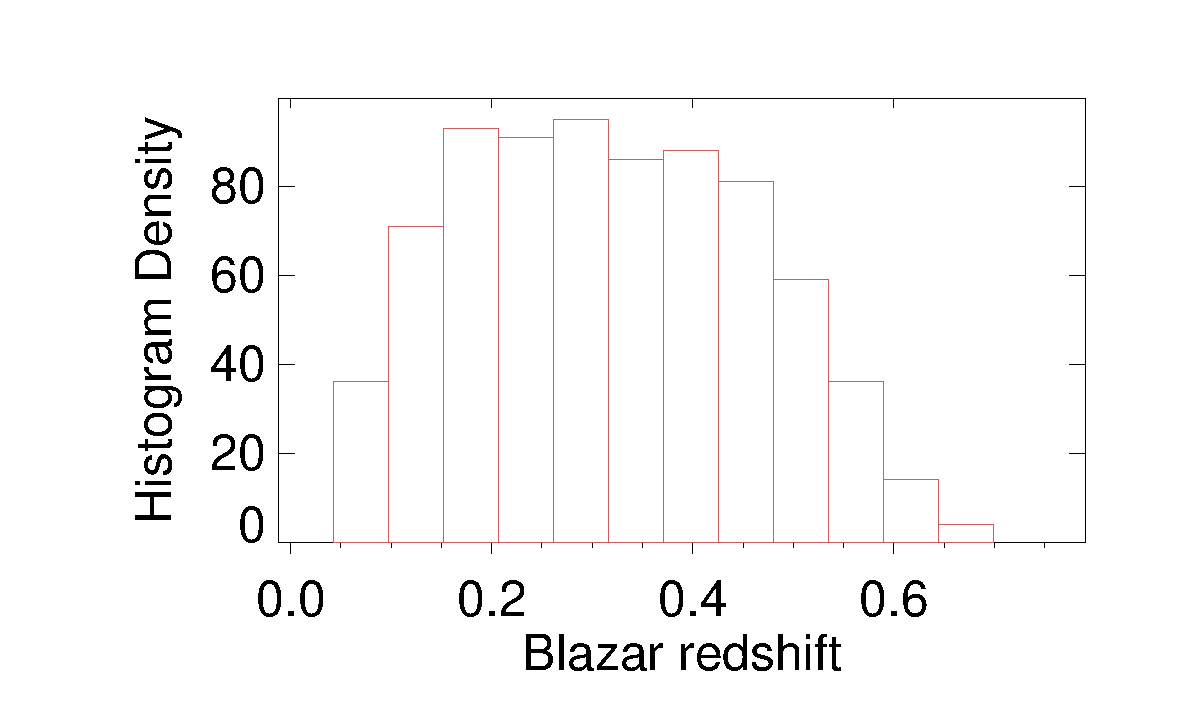
\includegraphics[width=3.5in]{blazar_zhist.eps}
\caption{Distribution of the redshifts for the 2335~blazars within the footprint of the SDSS DR8. Redshift information comes from the BzCat version 3.  
\label{fig-blazar_zhist}}
\end{figure}

The value of \bgb~is computed for each blazar in the Sloan field using Equation~\ref{eqn-bgb}. For the galaxy luminosity function, we use values of $\phi^*=5.33\times10^{-3}$~Mpc$^{-3}$, $M_r^*=-21.18$, and $\alpha=-1.05$, based on the SDSS luminosity function at $z=0.1$ \citep{bla03a}. The Schechter function is integrated between magnitudes of $M_r=28$ (lower values introduce numerical errors) and the counting magnitude of the blazar field. We do not assume any evolution of the LF as a function of redshift at this time.

Since this is not a targeted survey of the blazar fields, observations are not particularly deep and so the number of detected neighbors is low, especially at $z>0.1$. Assuming Poissionian statistics and requiring a S/N$>3$, results below are only for blazars with at least 10 detections of neighboring galaxies within 500~kpc. The final sample contains 757 blazars, with 528 BL~Lacs, 98 FSRQs, and 131 unclassified blazars. 


%%%%%%%%%%%%
%%% RESULTS
%%%%%%%%%%%%

\section{Results}\label{sec-survey_results}

\begin{figure*}
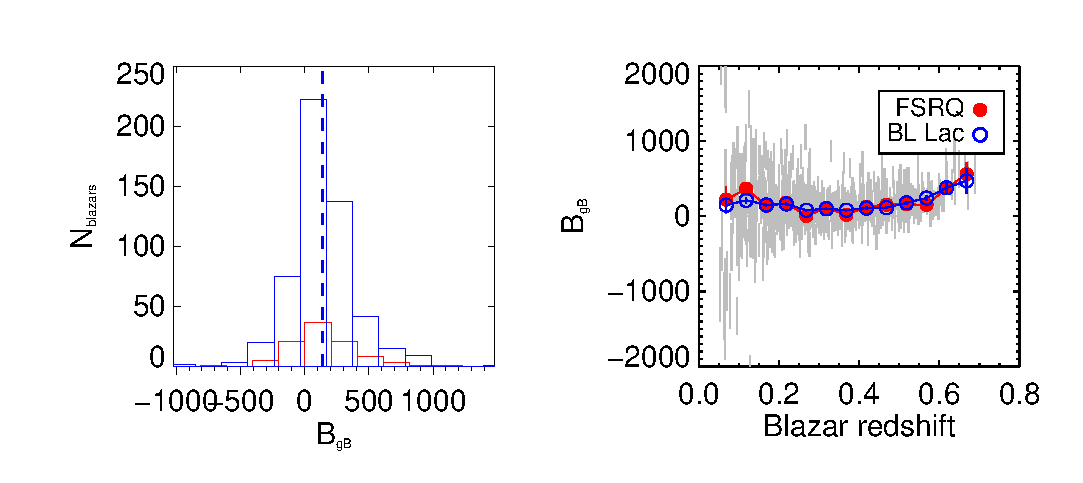
\includegraphics[width=7in]{bgb_blazars.eps}
\caption{Top left: Distribution of the \bgb~clustering amplitudes for the entire blazar sample. Top right: Distribution of \bgb~for the BL~Lac and FSRQ sub-populations. Bottom left: \bgb~as a function of the blazar redshift. Bottom right: \bgb~as a function of redshift, color-coded by blazar type. 
\label{fig-bgb_blazars}}
\end{figure*}

Figure~\ref{fig-bgb_blazars} shows the distribution of the clustering amplitudes for the blazars in our sample. The mean value for the blazars is $144\pm402$, confirming the basic conclusion that blazars tend to lie in overdense regions of the universe. 

Splitting the sample by blazar type, the clustering amplitudes are found to be remarkably similar. BL~Lacs in the sample have a mean \bgb~of $148\pm312$, while FSRQs have $144\pm268$. A Kolmogorov-Smirnov test confirms that these values are not inconsistent with being drawn from the same population at a probability of $0.274 (1.0\sigma)$. Therefore, there is no evidence based on the clustering statistics that BL~Lacs and FSRQs inhabit different environments at redshifts $z<0.75$. 

The effect of assuming an earlier cosmology ($q_0=0, \Omega_\Lambda=0, H_0=50~\mbox{km s}^{-1}\mbox{Mpc}^{-1}$) is to: CHECK THIS FOR COMPARISON. 

%%%%%%%%%%%%
%%% DISCUSSION
%%%%%%%%%%%%

\section{Discussion}\label{sec-survey_discussion}

\subsection{Comparison samples}\label{ssec-comparison}

We compare the clustering properties of blazars in our sample to active radio galaxies since, according to the unified model, these are the parent populations of blazars. As a result, the clustering properties of radio galaxies should be similar to those of blazars, assuming that the orientation of the jet has no effect on the megaparsec-scale environment. 

The largest pure morphological catalogue of radio galaxies is the 3CRR catalogue assembled by \citet{lai83}. More recent catalogues include the CoNFIG sample of \citet{gen08}, which combines images of galaxies from the NVSS and FIRST surveys.  Figure~\ref{fig-bgb_tcrr} shows the distribution of the clustering amplitudes for the radio galaxies. 

\citet{gen13} specifically measure the richness of the radio galaxy sample using the richness method of \citet{win11}. This alternative method might easily be adapted to the blazar sample. They found that FR~I galaxies existed in richer environments than FR~II galaxies.

\begin{figure*}
\includegraphics[width=7in]{bgb_tcrr.eps}
\caption{Top left: Distribution of the \bgb~clustering amplitudes for the radio galaxies in the 3CRR catalog. Top right: Distribution of \bgb~for FR~I and FR~II sub-populations. Bottom left: \bgb~as a function of the galaxy redshift. Bottom right: \bgb~as a function of redshift, color-coded by morphological type. 
\label{fig-bgb_tcrr}}
\end{figure*}

The TCRR sample has explicit morphologies determined by careful analysis, but is sorely lacking in sample size and redshift distribution. \citet{kim08} have identified a larger sample of radio galaxies with less precise morphology, but much greater size. We use their sample of galaxies cross-identified in four radio (FIRST, NVSS, WENSS, GB6) and one optical (SDSS) surveys with spectroscopic identification. Out of the 2886 galaxies in the Sloan footprint, $1964$ fall in the redshift range $0.162<z<0.75$; we match this to the redshift distribution of the blazars in bins of $\Delta z=0.05$. This reduces the number of galaxies to $XX$. 

We compute \bgb~for this sample using same method as for the BZCAT blazars. 

Recently, \citet{ram13} used the angular clustering amplitudes to compare intermediate-redshift ($z<0.7$) radio galaxies compared to type-2 quasars and quescent early-type galaxies. They found that radio galaxies live in significantly denser environments than quiescent galaxies, with average values of $B_{gq}=384\pm79$ for PRGs and $B_{gq}=111\pm21$ for quiescent galaxies.

\subsection{The blazar sequence/envelope}\label{ssec-sequence}

The concept of the blazar sequence has been called into question in recent years. \citet{pad07} demonstrated that the anti-correlation between \lpeak~and \nupeak~drastically decreases when selection effects of blazar surveys are taken into account. This, combined with the discovery of FSRQs peaking in the UV/X-ray bands \citep{pad03,lan08a} and the lack of high-frequency BL~Lacs, suggested that the simplest form of the blazar sequence has been ruled out. 

\citet{mey11} suggested a modification to the sequence in which blazars form two distinct populations in the \nupeak-\lpeak~plane. The two populations each form an upper edge to envelopes of progressively misaligned blazars; the parent populations of the two galaxies are related to `weak jet' (low kinetic powers with radiatively inefficient accretion) and `strong jet' sources (single Lorentz factor-jets with efficient accretion rates). The former population corresponds to FR~I radio galaxies and most BL~Lacs, while the latter corresponds to FR~II galaxies and most FSRQs. The observed properties of the two blazar populations overlap with those of radio galaxies as the jets become more misaligned, near \nupeak$\sim10^{13}$~Hz and $\nu$\lpeak$\sim10^{42}$~erg~s$^{-1}$. 

\citet{gio12} present an alternative explanation for the classification schemes of blazars in which their behavior in the \nupeak-\lpeak~plane is almost entirely due to selection effects, rather than jet alignment. Using Monte Carlo simulations of the observed properties of blazars, they posit that the measurement of optical emission lines -- a standard method for classifying BL~Lacs vs. FSRQs -- are strongly affected by the existence of continuum emission, and can be diluted or washed out completely for some jet strengths. This leads to the existence of high-\nupeak, radio-loud objects that do not appear in the characteristic plane because their redshift is not measurable. They also suggest that blazars represent two physically distinct classes of objects (similar to \citet{mey11}), in which the key difference is the efficiency of the accretion rate in the parent radio galaxy. 

Overdensities have also been reported for high-redshift radio galaxies by counting the number of IRAC \citep{gal12} and MIPS \citep{may12} sources around the location of the radio galaxy. Using a counts-in-cell analysis, both groups found moderate overdensities within 500~Mpc of the radio galaxy. This is interepreted as evidence that clusters and protoclusters are preferentially associated with radio-loud galaxies. 

New study of environments by \citet{ram13}. 

\subsection{Variability and environment}

We have also isolated several BL Lacs with unusually weak variability properties. One interpretation is that galaxies with low variability do not have the direction of ultra-high energy cosmic ray (UHECR) emission isotropized by the magnetic regions of surrounding galaxies \citep{raz12}. In that case, we would expect low-variability BL Lacs to occur in underdense regions, and thus have \bgb~values below the average for the BL Lac sample.  

Two BL Lacs with low variability (C.~Dermer, priv. comm.) have been identified within the SDSS coverage: 1ES~0229+200 ($z=0.14$) and RGB~J0152+017 ($z=0.08$). \bgb~values for these blazars are 1395 and 4068, respectively; these are well {\it above} the average \bgb~for BL~Lacs, and in fact fall above the 90th percentile. We note, however, that this is also consistent with the redshift-\bgb~relation observed in Figure~\ref{fig-bgb_blazars}. If we account for this dependence by looking at the mean \bgb~values for each redshift bin, both BL~Lacs have clustering amplitudes very close to the mean value at their respective redshift. Our results show no evidence that these low-variability objects differ in their environmental parameters.  

Idea: plot variability vs. \bgb? Sent email to Chuck Dermer asking about this. 

%%%%%%%%%%%%
%%% CONCLUSIONS
%%%%%%%%%%%%

\section{Conclusions}\label{sec_conclusions}

We have computed the clustering amplitude for a sample of nearly 3000 blazars, the largest amount for which these have been determined by more than an order of magnitude. 

%%%%%%%%%%%%
%%% ACKNOWLEDGMENTS
%%%%%%%%%%%%

%\acknowledgments
%

%\clearpage

%%%%%%%%%%%%
%%% BIBLIOGRAPHY
%%%%%%%%%%%%

\bibliography{mn-jour,kwrefs}

\bsp

\label{lastpage}

\end{document}
